\chapter{Client/Server}
\renewcommand{\chaptertitle}{Client/Server}

\lehead[]{\normalfont\sffamily\hspace*{-2.00cm}\textcolor{white}{\colorbox{lightblue}{\makebox[1.60cm][r]{\thechapter}}}\hspace{0.17cm}\textcolor{lightblue}{\chaptertitle}}
\rohead[]{\textcolor{lightblue}{\chaptertitle}\normalfont\sffamily\hspace*{0.17cm}\textcolor{white}{\colorbox{lightblue}{\makebox[1.60cm][l]{\thechapter}}}\hspace{-2.00cm}}
%\chead[]{}
\rehead[]{\textcolor{lightblue}{AvHG, Inf, My}}
\lohead[]{\textcolor{lightblue}{AvHG, Inf, My}}


\section{Client}

\subsection{Sockets}

Die Programmierschnittstelle zum Zugriff auf ein TCP/IP-Netz bezeichnet man als
Socket. Ein Socket ist stream-basiert, das heißt die Daten werden in einem
\glqq Strom\grqq\ von Bytes (ein Byte nach dem anderen) über das Netz geschickt
und in derselben Reihenfolge empfangen.

Ein Client-Programm nimmt Verbindung zu einem Server auf, in dem es ein Objekt
der Klasse \myClass{Socket} aus dem Package \myPackage{java.net} erzeugt. Im
Konstruktor wird die Rechner-Adresse (IP-Name, Domain-Name oder
\myClass{InetAddress}-Objekt) und die Port-Nummer des Servers angegeben:

\begin{lstlisting}
public Socket(String host, int port) throws UnknownHostException, IOException
\end{lstlisting}

oder

\begin{lstlisting}
public Socket(InetAddress address, int port) throws IOException
\end{lstlisting}

Wenn die Rechner-Adresse nicht aufgelöst werden konnte, wird eine
\myClass{UnknownHostException} erzeugt. Wenn der Socket nicht geöffnet werden
konnte, wird eine \myClass{IOException} erzeugt.

\subsection{Streams}

Nachdem die Socket-Verbindung erfolgreich aufgebaut wurde, kann mit den beiden
Methoden \lstinline|getInputStream()| und \lstinline|getOutputStream()| je ein
Stream zum Empfangen und zum Senden von Daten beschafft werden. Um Streams
verwenden zu können, muss das Package \myPackage{java.io} importiert werden.

\begin{lstlisting}
public InputStream getInputStream() throws IOException
public OutputStream getOutputStream() throws IOException
\end{lstlisting}

Man könnte direkt mit diesen beiden Streams arbeiten, um Daten über das
Netzwerk zu lesen bzw.\ zu schreiben. Aber das ist nicht zu empfehlen (zumindest
dann nicht, wenn nicht nur Binärdaten in Form von einzelnen Bytes, sondern
Zeichen bzw. Texte verschickt werden sollen). Besser ist es das
\myClass{OutputStream}-Objekt in einen \myClass{OutputStreamWriter} und das
\myClass{InputStream}-Objekt in einen \myClass{InputStreamReader} zu verpacken.
Das bietet nämlich den Vorteil, dass man die Kodierung des Zeichensatzes
festlegen kann.

\begin{lstlisting}
public InputStreamReader(InputStream is, String charsetName) 
        throws UnsupportedEncodingException
public OutputStreamWriter(OutputStream os, String charsetName) 
        throws UnsupportedEncodingException
\end{lstlisting}

\begin{center}
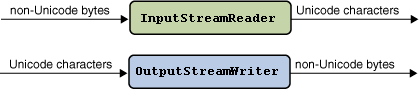
\includegraphics[width=0.7\textwidth]{./inf/SEKII/43_Java_ClientServer/StreamEncoding.png}
% http://docs.oracle.com/javase/tutorial/i18n/text/stream.html
% copyright??
\end{center}

Sollen hingegen Binärdaten gelesen und geschrieben werden, dann arbeitet man
direkt mit dem \myClass{InputStream}- bzw.\ \myClass{OutputStream}-Objekten
(wird bei uns im Unterricht nicht vorkommen).

\subsection{Einlesen von Daten}

Zum Lesen von Daten aus dem Stream besitzt die Klasse
\myClass{InputStreamReader} unter anderem die folgende Methode:

\begin{lstlisting}
public int read() throws IOException
\end{lstlisting}

\lstinline|read()| liest das nächste Zeichen vom Datenstrom ein. Wenn ein
Zeichen übertragen wurde, ist das Ergebnis eine Zahl, die mit einem Type-Cast
in einen Buchstaben (\lstinline|char|) umgewandelt werden kann. Falls keine
Daten verfügbar sind, blockiert die Methode bis das nächste Zeichen angekommen
ist. Wenn die Datenverbindung geschlossen wurde, wird die Zahl \lstinline|-1|
zurückgegeben.

\subsection{Beispiel: Einlesen von Daten aus einem Socket (Code-Auszug)}

\begin{lstlisting}
int zeichen;
String text = "";
try (Socket socket = new Socket ("localhost", 12345)) {
    InputStreamReader in = new InputStreamReader(socket.getInputStream(), "UTF-8"); 
    while ((zeichen = in.read()) != -1) {
        text += (char) zeichen;
        System.out.println(text);
    }	
} catch (Exception e) {
    System.out.println("Fehler: " + e.getMessage());
}
\end{lstlisting}

\subsection{Ausgabe von Daten}

Zur Ausgabe von Daten besitzt die Klasse \myClass{OutputStreamWriter} unter
anderem die folgenden Methoden:

\begin{lstlisting}
public void write(int zeichen) throws IOException
public void write(String text) throws IOException
\end{lstlisting}

Die erste Variante der \lstinline|write()|-Methode schreibt ein einzelnes
Zeichen in den Datenstrom, die untere Variante schreibt einen String. Die mit
\lstinline|write()| geschriebenen Daten werden zunächst (intern)
zwischengepuffert und erst dann tatsächlich verschickt, wenn der Puffer gefüllt
ist. Mit der Methode \lstinline|flush()| kann man das tatsächliche Versenden
sofort erzwingen:

\begin{lstlisting}
public void flush() throws IOException
\end{lstlisting}

Beispiel für die Verwendung der Methoden:

\begin{lstlisting}
String text = "Hallo";
try (Socket socket = new Socket ("localhost", 12345)) {
    OutputStreamWriter out = new OutputStreamWriter(socket.getOutputStream(), "UTF-8");
    out.write(text);
    out.write(System.lineSeparator());         æ// Zeilenumbruch senden
    æout.flush();
} catch (Exception e) {
    System.out.println("Fehler: " + e.getMessage());
}
\end{lstlisting}

\subsection{Verbindung beenden}

Nach Ende der Kommunikation sollte der Socket selbst mit der Methode
\lstinline|close()| geschlossen werden:

\begin{lstlisting}
public void close() throws IOException
\end{lstlisting}

Durch das Schließen des Sockets werden auch der In- und OutputStream mit
geschlossen.


\section{Server}

Die Programmierung eines Servers funktioniert ganz ähnlich wie die eines
Clients. Lediglich der Verbindungsaufbau ist etwas komplizierter:

Ein Server muss in der Lage sein mit beliebig vielen Clients gleichzeitig zu
kommunizieren. Für jede Client-Verbindung benötigt er einen eigenen Socket.
Wenn der Server gestartet wird, öffnet er einen Haupt-Socket, in dem er auf
eingehende Verbindungen wartet. Für jede aufgebaute Verbindung generiert das
System einen neuen Socket, damit der Haupt-Socket für weitere \glqq Anrufe\grqq\
frei bleibt.

Den Haupt-Socket eines Servers generiert man mit der Klasse
\myClass{ServerSocket} aus dem Package \myPackage{java.net}. Wichtig sind der
Konstruktor der Klasse und die Methode \lstinline|accept()|:

\begin{lstlisting}
public ServerSocket(int port)   æ// erzeugt Haupt-Socket mit angegebener Port-Nummer 
æpublic Socket accept()	        æ// wartet auf eingehende Verbindungen
\end{lstlisting}

Die Methode \lstinline|accept()| blockiert so lange, bis sich ein Client bei der
Server-Anwendung meldet. Ist der Verbindungsaufbau erfolgt, liefert
\lstinline|accept()| ein \myClass{Socket}-Objekt zurück, das zur
Kommunikation mit dem Client verwendet werden kann.

Beispiel-Code (Auszug)

\begin{lstlisting}
try (ServerSocket serverSocket = new ServerSocket(12345)) {
   while (true) {
       Socket clientSocket = serverSocket.accept();
       OutputStreamWriter out = 
               new OutputStreamWriter(clientSocket.getOutputStream(), "UTF-8");
       String text = "Hallo!";
       out.write(text);
       out.flush();
       clientSocket.close();
   }
} catch(Exception e) {
    System.out.println("Fehler: " + e.getMessage());
}
\end{lstlisting}


\section{Allgemeiner Aufbau von Client- und Server-Programmen}

Sowohl Clients als auch Server haben fast immer den gleichen Aufbau. 

\begin{compactitem}
\item Clients brauchen neben der Klasse für das Anwendungsfenster eine
Thread-Klasse, in der auf eingehende Daten vom Server reagiert werden kann.

\item Server haben im Vergleich zum Client üblicherweise ein deutlich weniger
komplexes User-Interface (Anwendungsfenster) oder verzichten gar ganz auf ein
solches. Dafür brauchen sie zwei Thread-Klassen. Im Haupt-Thread wartet der
Server auf eingehende Verbindungswünsche von Clients. Dazu erstellt er zunächst
einen Server-Socket und \glqq horcht\grqq\ auf diesem auf eingehende
Verbindungen. Sobald solch eine Verbindung zustande kommt erzeugt der
Haupt-Thread einen normalen Socket und übergibt diesen für die weitere
Kommunikation der zweiten Thread-Klasse: dem Client-Thread. Der Haupt-Thread
ist jetzt wieder frei für weitere Clients. Auf diese Weise kann ein Server mit
quasi beliebig vielen Clients gleichzeitig kommunizieren. Für jede
Client-Verbindung wird dann jeweils ein eigener Client-Thread erzeugt.
\end{compactitem}

Im Folgenden ist ein Gerüst für Client und Server gegeben. Es ist noch ohne
echte Funktionalität. Zwar wird eine Verbindung aufgebaut (Sockets, sowie
InputStreams und OutputStreams auf Server- und Client-Seite erstellt), aber es
ist noch kein Protokoll implementiert.

Genau darin: In der Implementierung des jeweiligen Protokoll liegt eure
eigentliche Arbeit!

Neben der Implementierung des Protokolls muss oft noch anderes geleistet
werden: Bei schreibenden Dateizugriffen sowie schreibenden Zugriffen auf
Textfelder und andere Elemente des Anwendungsfensters muss sichergestellt
werden, dass nicht mehrere Threads gleichzeitig die selben Daten verändern
wollen. Dies muss über einen geeignet gewählten \emph{Monitor} in einem
\lstinline|synchronized|-Block gewährleistet werden.

\subsection{Tipps}

\begin{compactitem}
\item Nehmt euch ausreichend Zeit um das Protokoll zu verstehen! Da die
Umsetzung des Protokolls der schwierigste Teil der Client/Server-Programmierung
ist, lohnt es sich zunächst mit Stift und Papier die verschiedenen Nachrichten
des Protokolls aufzuschreiben und zu strukturieren. Danach wird euch die
Implementierung im Programm erheblich leichter fallen!

\item Testet immer gegen einen bestehenden (und verlässlich funktionierenden)
\glqq Gegenspieler\grqq . Bei Aufgaben, in denen sowohl Client- als auch Server
entwickelt werden sollen, ist es extrem ratsam, zunächst gegen einen bereits
vorhandenen (vom Lehrer zur Verfügung gestellten) Server oder Client zu testen.
Wenn ihr zuerst den Client entwickeln wollt, dann testet ihr gegen den Server
den ihr vom Lehrer bekommen habt. Und umgekehrt. Ansonsten werdet ihr mit
Sicherheit viel Zeit und Nerven lassen. Mit einem halbfertigen Client gegen
einen halbfertigen Server zu testen macht keinen Spaß!

\item In \lstinline|catch|-Blöcken unbedingt immer mit
\lstinline|e.printStackTrace()| die komplette Fehlermeldung ausgeben lassen.
Dort wird euch neben dem Fehlertext sogar ein Hinweis auf die konkrete Stelle
in eurer Java-Datei gegeben, in der die Ausnahme (Exception) erzeugt wurde.
Dies nicht zu tun ist fahrlässig und kostet euch im Zweifelsfall viel Zeit und
Punkte!

\item \glqq Sprechende\grqq\ Bezeichner verwenden. \lstinline|btnSenden| ist
erheblich aussagekräftiger als \lstinline|button3|! Genau so wie
\lstinline|serverName| instruktiver ist als \lstinline|text|!
\end{compactitem}

\subsection{Server-Gerüst}

Datei \myFile{Server.java}:

\begin{lstlisting}
import java.awt.*;
import java.awt.EventQueue;
import javax.swing.*;
import javax.swing.border.EmptyBorder;

public class Server extends JFrame {
    æ// globale Variablen
    æprivate static final int WIDTH = 300;
    private static final int HEIGHT = 300;
    private HauptThread thread;

    public Server(final String title) {
        super(title);
        setDefaultCloseOperation(JFrame.EXIT_ON_CLOSE);
        JPanel contentPane = new JPanel();
        contentPane.setBorder(new EmptyBorder(5, 5, 5, 5));
        contentPane.setLayout(new BorderLayout(0, 0));
        contentPane.setPreferredSize(new Dimension(WIDTH, HEIGHT));
        setContentPane(contentPane);
        pack();
        setLocationRelativeTo(null);
        setResizable(false);
        setVisible(true);
		
        thread = new HauptThread();
        thread.start();
    }
	
    public static void main(final String[] args) {
        EventQueue.invokeLater(new Runnable() {
            @Override
            public void run() {
                try {
                    new Server("Server");
                } catch (Exception e) {
                    e.printStackTrace();
                }
            }
        });
    }
}
\end{lstlisting}

\vfill

Datei \myFile{HauptThread.java}

\begin{lstlisting}
import java.net.*;

public class HauptThread extends Thread {
    æ// Die Aufgabe des Hauptthreads ist es, auf eingehende Verbindungswünsche
    // von Clients zu warten und diese dann mit einem Client-Socket zu
    // "versorgen".
    // Sobald dies geschehen ist wird der Client-Thread gestartet (dieser
    // bekommt den Client-Socket als Parameter übergeben).

    æpublic HauptThread() {
        æ// Hier muss normalerweise nichts getan werden.
    æ}

    @Override
    public void run() {
        try (ServerSocket serverSocket = new ServerSocket(22222)) {
            while (true) {
                Socket socket = serverSocket.accept();
                ClientThread client = new ClientThread(socket);
                client.start();
            }
        } catch (Exception e) {
            e.printStackTrace();
        }
    }
}
\end{lstlisting}

\subsubsection{Anmerkung}

Die HaupThread-Klasse kann so in den meisten Fällen fast oder völlig
unverändert benutzt werden!

\pagebreak

Datei \myFile{ClientThread.java}

\begin{lstlisting}
import java.net.*;
import java.io.*;

public class ClientThread extends Thread {
    private Socket socket;
    private InputStreamReader in;
    private OutputStreamWriter out;

    public ClientThread(Socket sock) {
        this.socket = sock;
        try {
            in = new InputStreamReader(socket.getInputStream(), "UTF-8");
            out = new OutputStreamWriter(socket.getOutputStream(), "UTF-8");
        } catch (UnsupportedEncodingException e) {
            e.printStackTrace();
        } catch (IOException e) {
            e.printStackTrace();
        }
    }

    @Override
    public void run() {
        try {
            int zeichen;
            while ((zeichen = in.read()) != -1) {
                æ// Hier werden die Daten vom Client gelesen und verarbeitet
                // (InputStream)
                // und Daten zum Client geschickt (OutputStream)
                // Was hier tatsächlich zu tun ist wird durch das Protokoll
                // definiert

                // Das ist eure eigentliche Arbeit!
            æ}
            æ// Die Verbindung (InputStream des Servers bzw. OutputStream des
            // Clients wurde vom Client getrennt --> in.read() == -1
            // Jetzt muss nur noch aufgeräumt werden (der Socket - und indirekt
            // damit auch die Streams - werden geschlossen).
            æsocket.close();
        } catch (Exception e) {
            e.printStackTrace();
        }
    }
}
\end{lstlisting}

\subsubsection{Anmerkung}

Die Übungsaufgabe zum Rechentrainer stellt einen Sonderfall dar, in so fern,
als dort der Server nicht darauf wartet, dass der Client die Verbindung beendet

\begin{lstlisting}
while ( (zeichen = in.read()) != -1 )
\end{lstlisting}
   
sondern vielmehr seinerseits mit zählt und nach fünf erfolgreich gelösten
Aufgaben die Verbindung beendet:

\begin{lstlisting}
for (int i = 0; i < 5; i++) {
    aufgabeSenden();
    antwortLesen();
}
\end{lstlisting}

\subsection{Client-Gerüst}

Datei \myFile{Client.java}

\begin{lstlisting}
import java.awt.*;
import java.awt.event.*;
import java.io.*;
import java.net.Socket;
import javax.swing.*;
import javax.swing.border.EmptyBorder;

public class Client extends JFrame {
    // globale Variablen
    private static final int WIDTH = 500;
    private static final int HEIGHT = 400;
    private JTextField tfServer, tfStatus, tfEingabe;
    private JButton btnVerbinden, btnTrennen, btnSenden;
    JTextArea textAreaAusgabe;
    private boolean verbunden = false;
    Socket socket;
    InputStreamReader in;
    private OutputStreamWriter out;
    private LeseThread thread;

    public Client(final String title) {
        æsuper(title);
        setDefaultCloseOperation(JFrame.EXIT_ON_CLOSE);
        JPanel contentPane = new JPanel();
        contentPane.setBorder(new EmptyBorder(10, 10, 10, 10));
        contentPane.setPreferredSize(new Dimension(WIDTH, HEIGHT));
        setContentPane(contentPane);
        GridBagLayout gbl_contentPane = new GridBagLayout();
        gbl_contentPane.columnWidths = new int[] { 26, 322, 0, 0 };
        gbl_contentPane.rowHeights = new int[] { 0, 0, 0, 0, 0, 0 };
        gbl_contentPane.columnWeights = new double[] { 1.0, 1.0, 0.0, 
        											Double.MIN_VALUE };
        gbl_contentPane.rowWeights = new double[] { 0.0, 0.0, 0.0, 0.0, 1.0,  
                                                    Double.MIN_VALUE };
        contentPane.setLayout(gbl_contentPane);

        JLabel lblServer = new JLabel("Server:");
        GridBagConstraints gbc_lblServer = new GridBagConstraints();
        gbc_lblServer.anchor = GridBagConstraints.EAST;
        gbc_lblServer.insets = new Insets(0, 0, 5, 5);
        gbc_lblServer.gridx = 0;
        gbc_lblServer.gridy = 0;
        contentPane.add(lblServer, gbc_lblServer);

        tfServer = new JTextField();
        GridBagConstraints gbc_tfServer = new GridBagConstraints();
        gbc_tfServer.insets = new Insets(0, 0, 5, 5);
        gbc_tfServer.fill = GridBagConstraints.HORIZONTAL;
        gbc_tfServer.gridx = 1;
        gbc_tfServer.gridy = 0;
        contentPane.add(tfServer, gbc_tfServer);
        tfServer.setColumns(10);

        btnVerbinden = new JButton("verbinden");
        btnVerbinden.addActionListener(new ActionListener() {
            public void actionPerformed(ActionEvent e) {
                verbinden();
            }
        });
        GridBagConstraints gbc_btnVerbinden = new GridBagConstraints();
        gbc_btnVerbinden.insets = new Insets(0, 0, 5, 0);
        gbc_btnVerbinden.gridx = 2;
        gbc_btnVerbinden.gridy = 0;
        contentPane.add(btnVerbinden, gbc_btnVerbinden);

        JLabel lblStatus = new JLabel("Status:");
        GridBagConstraints gbc_lblStatus = new GridBagConstraints();
        gbc_lblStatus.anchor = GridBagConstraints.EAST;
        gbc_lblStatus.insets = new Insets(0, 0, 5, 5);
        gbc_lblStatus.gridx = 0;
        gbc_lblStatus.gridy = 1;
        contentPane.add(lblStatus, gbc_lblStatus);

        tfStatus = new JTextField();
        tfStatus.setEditable(false);
        GridBagConstraints gbc_tfStatus = new GridBagConstraints();
        gbc_tfStatus.insets = new Insets(0, 0, 5, 5);
        gbc_tfStatus.fill = GridBagConstraints.HORIZONTAL;
        gbc_tfStatus.gridx = 1;
        gbc_tfStatus.gridy = 1;
        contentPane.add(tfStatus, gbc_tfStatus);
        tfStatus.setColumns(10);

        btnTrennen = new JButton("trennen");
        btnTrennen.setEnabled(false);
        btnTrennen.addActionListener(new ActionListener() {
            public void actionPerformed(ActionEvent e) {
                trennen();
            }
        });
        GridBagConstraints gbc_btnTrennen = new GridBagConstraints();
        gbc_btnTrennen.fill = GridBagConstraints.HORIZONTAL;
        gbc_btnTrennen.insets = new Insets(0, 0, 5, 0);
        gbc_btnTrennen.gridx = 2;
        gbc_btnTrennen.gridy = 1;
        contentPane.add(btnTrennen, gbc_btnTrennen);

        JLabel lblEingabe = new JLabel("Eingabe:");
        GridBagConstraints gbc_lblEingabe = new GridBagConstraints();
        gbc_lblEingabe.anchor = GridBagConstraints.EAST;
        gbc_lblEingabe.insets = new Insets(0, 0, 5, 5);
        gbc_lblEingabe.gridx = 0;
        gbc_lblEingabe.gridy = 2;
        contentPane.add(lblEingabe, gbc_lblEingabe);

        tfEingabe = new JTextField();
        GridBagConstraints gbc_tfEingabe = new GridBagConstraints();
        gbc_tfEingabe.insets = new Insets(0, 0, 5, 5);
        gbc_tfEingabe.fill = GridBagConstraints.HORIZONTAL;
        gbc_tfEingabe.gridx = 1;
        gbc_tfEingabe.gridy = 2;
        contentPane.add(tfEingabe, gbc_tfEingabe);
        tfEingabe.setColumns(10);

        btnSenden = new JButton("senden");
        btnSenden.setEnabled(false);
        btnSenden.addActionListener(new ActionListener() {
            public void actionPerformed(ActionEvent e) {
                senden();
            }
        });
        GridBagConstraints gbc_btnSenden = new GridBagConstraints();
        gbc_btnSenden.fill = GridBagConstraints.HORIZONTAL;
        gbc_btnSenden.insets = new Insets(0, 0, 5, 0);
        gbc_btnSenden.gridx = 2;
        gbc_btnSenden.gridy = 2;
        contentPane.add(btnSenden, gbc_btnSenden);

        JLabel lblAusgabe = new JLabel("Ausgabe:");
        GridBagConstraints gbc_lblAusgabe = new GridBagConstraints();
        gbc_lblAusgabe.anchor = GridBagConstraints.EAST;
        gbc_lblAusgabe.insets = new Insets(0, 0, 5, 5);
        gbc_lblAusgabe.gridx = 0;
        gbc_lblAusgabe.gridy = 3;
        contentPane.add(lblAusgabe, gbc_lblAusgabe);

        JScrollPane scrollPane = new JScrollPane();
        GridBagConstraints gbc_scrollPane = new GridBagConstraints();
        gbc_scrollPane.gridwidth = 3;
        gbc_scrollPane.insets = new Insets(0, 0, 0, 5);
        gbc_scrollPane.fill = GridBagConstraints.BOTH;
        gbc_scrollPane.gridx = 0;
        gbc_scrollPane.gridy = 4;
        contentPane.add(scrollPane, gbc_scrollPane);

        textAreaAusgabe = new JTextArea();
        scrollPane.setViewportView(textAreaAusgabe);

        pack();
        setLocationRelativeTo(null);
        setResizable(false);
        setVisible(true);
    æ}

    public void verbinden() {
        æ// Die Verbindung zum Server wird aufgebaut.
        // InputStreamReader und OutputStreamWriter des Sockets werden
        // geholt.
        // Anschließend wird der InputStreamReader an den Lesethread
        // übergeben und dieser gestartet.

        ætry {
            if (!verbunden) {
                verbunden = true;
                String serverName = tfServer.getText();
                socket = new Socket(serverName, 22222);
                System.out.println("Verbindung hergestellt!");
                in = new InputStreamReader(socket.getInputStream(), "UTF-8");
                out = new OutputStreamWriter(socket.getOutputStream(), "UTF-8");
                thread = new LeseThread(this, in);
                thread.start();
                tfServer.setEnabled(false);
                btnVerbinden.setEnabled(false);
                btnTrennen.setEnabled(true);
                btnSenden.setEnabled(true);
                tfStatus.setText("verbunden");
            }
        } catch (Exception exc) {
            tfStatus.setText("Fehler: " + exc.getMessage());
            tfServer.setEnabled(true);
            btnVerbinden.setEnabled(true);
            btnTrennen.setEnabled(false);
            btnSenden.setEnabled(false);
            tfStatus.setText("getrennt");
            verbunden = false;
        }
    }

    public void senden() {
        if (verbunden) {
            try {
                æ// Was hier gesendet wird (und auch wodurch das Senden
                // ausgelöst wird) wird durch das Protokoll definiert!
                //
                // ACHTUNG: Je nach Definition des Protokolls kann das
                // Senden auch unabhängig von Benutzereingaben geschehen.
                // Etwa als automatisierte Reaktion auf eine Anfrage vom
                // Server. In diesem Fall würde dies vermutlich im Lesethread
                // geschehen. Dieser müsste dann neben dem InputStreamReader-
                // auch das OutputStreamWriter-Objekt als Parameter 
                // übergeben bekommen.
            æ} catch (Exception exc) {
                textAreaAusgabe.append("Fehler: " + exc.getMessage());
            }
        }
    }

    public void trennen() {
        System.out.println("trennen");
        try {
            socket.close();
            tfStatus.setText("getrennt");
            tfServer.setEnabled(true);
            btnVerbinden.setEnabled(true);
            btnTrennen.setEnabled(false);
            btnSenden.setEnabled(false);
            verbunden = false;
        } catch (Exception exc) {
            tfStatus.setText("Fehler: " + exc.getMessage());
        }
    }

    public static void main(final String[] args) {
        EventQueue.invokeLater(new Runnable() {
            public void run() {
                try {
                    new Client("Client");
                } catch (Exception e) {
                    e.printStackTrace();
                }
            }
        });
    }
}
\end{lstlisting}

\subsubsection{Anmerkungen}

Die Datei \myFile{Client.java} ist zwar mit Abstand die Größte, aber für euch
vermutlich nicht die Schwierigste! Sie ist nur deshalb so groß, weil hier das
User-Interface implementiert wird.

Die anspruchsvollere Arbeit steckt in der \lstinline|while|-Schleife im
Lese-Thread. Dort wird ein Großteil des Protokolls implementiert!

Datei \myFile{LeseThread.java}

\begin{lstlisting}
import java.io.InputStreamReader;

public class LeseThread extends Thread {

    private Client main;
    private InputStreamReader in;

    public LeseThread(Client main, InputStreamReader in) {
        this.main = main;
        this.in = in;
    }

    @Override
    public void run() {
        int zeichen;
        try {
            while ((zeichen = in.read()) != -1) {
                æ// Hier werden die Daten vom Server gelesen und verarbeitet
                // (InputStream)
                // Was hier tatsächlich zu tun ist wird durch das Protokoll
                // definiert

                // Das ist eure eigentliche Arbeit!

            æ}
        } catch (Exception e) {
            e.printStackTrace();
        }
        try {
            main.socket.close();
        } catch (Exception e) {
            e.printStackTrace();
        }
    }
}
\end{lstlisting}